\chapter{The Data-Science Workflow}
\label{chap:workflow}
\chapterguide
  {No prior data-science experience is required. Basic familiarity with files and folders is helpful.}
  {distinguish data science from programming; frame answerable questions; inspect a dataset; and structure a reproducible R analysis.}

\section{Data science starts with a decision or question}
A useful analysis begins before code. A data scientist translates a broad concern into a question that can be answered with observable variables.

\begin{dstable}
\begin{tabularx}{\linewidth}{@{}p{3.1cm}p{4.0cm}X@{}}
\toprule
\rowcolor{DSPaleBlue!92}
Question type & Example & Typical evidence \\
\midrule
Descriptive & What does the dataset contain? & counts, distributions, summaries \\
Comparative & How do groups differ? & group summaries, intervals, tests \\
Relational & Which variables move together? & scatterplots, correlation, regression \\
Predictive & Can we estimate an unknown outcome? & holdout predictions and error metrics \\
Structural & Are there natural groups or lower-dimensional patterns? & clusters, principal components \\
\bottomrule
\end{tabularx}
\end{dstable}

\begin{pitfall}
A dataset does not automatically define the question. Starting with ``What can I do with these columns?'' often creates technically correct but irrelevant analysis. State the question first, then identify the evidence needed to answer it.
\end{pitfall}


\section{From a broad topic to an estimable quantity}
Broad topics become data-science problems only after the analyst specifies \emph{who or what is being studied}, \emph{what is measured}, and \emph{what quantity should be learned}. This quantity is sometimes called an \term{estimand}: the numerical or structural target that connects the question to evidence.

For example, ``Are flowers different?'' is too vague. ``How much does mean petal length differ among the three species represented in this dataset?'' identifies the unit of observation, the grouping variable, the outcome, and the comparison. A predictive version would be different again: ``How accurately can species be predicted for unseen flowers using the four measurements?''

\begin{utpfig}[Question-to-evidence ladder]{A strong analysis makes every transition explicit. If a link is vague, later modelling sophistication cannot repair the ambiguity.}{fig:question-evidence-ladder}
\begin{tikzpicture}[node distance=0.85cm]
\node[fcbox,text width=8.7cm] (context) {Context: what decision, scientific concern, or operational need motivates the work?};
\node[fcbox,text width=8.7cm,below=of context] (question) {Question: what exactly should be learned, compared, predicted, or discovered?};
\node[fcbox,text width=8.7cm,below=of question] (unit) {Unit + population: what does one row represent, and to which cases should conclusions apply?};
\node[fcbox,text width=8.7cm,below=of unit] (vars) {Variables + estimand: which measurements and which target quantity answer the question?};
\node[fcbox,text width=8.7cm,below=of vars] (method) {Method + validation: what analysis produces credible evidence and how will error be checked?};
\node[fcbox,text width=8.7cm,below=of method] (claim) {Claim: what can be stated, with uncertainty and limitations, without exceeding the design?};
\draw[fcedge] (context)--(question); \draw[fcedge] (question)--(unit); \draw[fcedge] (unit)--(vars); \draw[fcedge] (vars)--(method); \draw[fcedge] (method)--(claim);
\end{tikzpicture}
\end{utpfig}

\begin{keyidea}
The unit of observation is one of the most important pieces of metadata in a dataset. If a row represents a patient visit rather than a patient, then row counts, train/test splitting, and uncertainty calculations may need to account for repeated observations from the same person.
\end{keyidea}

\section{A practical analytical cycle}
\begin{utpfig}[Analytical cycle]{A good workflow is iterative rather than a straight line. Quality problems found during exploration can send the analyst back to preparation or even to the original question.}{fig:analytical-cycle}
\begin{tikzpicture}[node distance=1.2cm and 1.25cm]
\node[fcbox,text width=2.6cm] (q) {Question\\and context};
\node[fcbox,text width=2.6cm,right=of q] (d) {Acquire and\\understand data};
\node[fcbox,text width=2.6cm,right=of d] (p) {Prepare and\\audit};
\node[fcbox,text width=2.6cm,below=of p] (e) {Explore and\\visualise};
\node[fcbox,text width=2.6cm,left=of e] (m) {Model and\\quantify};
\node[fcbox,text width=2.6cm,left=of m] (c) {Validate and\\communicate};
\draw[fcedge] (q)--(d); \draw[fcedge] (d)--(p); \draw[fcedge] (p)--(e); \draw[fcedge] (e)--(m); \draw[fcedge] (m)--(c);
\draw[fcedge] (e.west) to[bend left=20] (d.south);
\draw[fcedge] (c.north) to[bend left=25] (q.south);
\end{tikzpicture}
\end{utpfig}


\section{The same dataset can support several kinds of analysis}
The question determines the role of each column. In the Iris data, \rcode{Species} is a grouping variable in a descriptive comparison, but becomes the target in a classification task. The four measurements can be outcomes in one analysis and predictive features in another.

\begin{utpfig}[Variable roles depend on the question]{Roles such as feature, target, identifier, and grouping variable are analytical roles, not permanent properties of a column.}{fig:variable-roles}
\begin{tikzpicture}[x=1cm,y=1cm]
\node[fcbox,text width=3.0cm] (data) at (0,1.7) {Same Iris table};
\node[fcbox,text width=3.5cm] (desc) at (-4.0,0) {Descriptive question\\Species = group\\Petal length = outcome};
\node[fcbox,text width=3.5cm] (pred) at (0,0) {Predictive question\\Species = target\\Measurements = features};
\node[fcbox,text width=3.5cm] (struct) at (4.0,0) {Structural question\\Measurements = geometry\\Species withheld};
\draw[fcedge] (data)--(desc); \draw[fcedge] (data)--(pred); \draw[fcedge] (data)--(struct);
\end{tikzpicture}
\end{utpfig}

\section{Rows, columns, and analytical roles}
A rectangular dataset usually stores one \term{observation} per row and one \term{variable} per column. Variables can play different analytical roles: identifiers locate records; features describe them; a target is the outcome to predict; metadata records context such as time or source.

The bundled Iris dataset contains 153 rows, four numeric measurements, one species label, and an identifier. Its small quality issues are useful later because even familiar teaching datasets should be audited rather than assumed perfect. The first inspection should answer shape, names, types, missingness, and basic range questions before any model is fitted.

\begin{lstlisting}[style=dsr]
iris <- read.csv("all_datasets/iris_dataset.csv")
dim(iris)
names(iris)
str(iris)
summary(iris)
\end{lstlisting}


\section{Three layers of reproducibility}
Reproducibility is easier to reason about when separated into three layers. \textbf{Computational reproducibility} asks whether the code reruns. \textbf{Analytical reproducibility} asks whether another analyst can understand and repeat the decisions: filters, transformations, metrics, and model settings. \textbf{Scientific reproducibility} asks whether a result persists with new data or a new sample from the intended population.

A script that runs but silently drops rows is computationally reproducible yet analytically weak. A well-documented analysis that cannot generalise beyond one convenience sample may be reproducible but still limited scientifically.

\begin{utpfig}[Reproducibility layers]{A professional workflow records enough information to reproduce both the computation and the reasoning, while recognising that new data provide the strongest test of generalisation.}{fig:repro-layers}
\begin{tikzpicture}[x=1cm,y=1cm]
\node[fcbox,text width=3.1cm] (comp) at (-3.7,0) {Computational\\same files + code\\same result};
\node[fcbox,text width=3.1cm] (anal) at (0,0) {Analytical\\same rules + assumptions\\same reasoning};
\node[fcbox,text width=3.1cm] (sci) at (3.7,0) {Scientific\\new sample/data\\similar conclusion?};
\draw[fcedge] (comp)--(anal); \draw[fcedge] (anal)--(sci);
\end{tikzpicture}
\end{utpfig}

\section{Reproducibility is part of the result}
An analysis is reproducible when another person can rerun the saved code against the stated data and obtain the same outputs. Keep the project structure predictable:

\begin{utpfig}[Course project structure]{The data are read-only inputs. Executable lab scripts live separately so code, data, and generated outputs do not become mixed together.}{fig:project-structure}
\begin{tikzpicture}[x=1cm,y=1cm]
\node[fcbox,text width=4.2cm] (root) at (0,1.5) {DATA SCIENCE/};
\node[fcbox,text width=3.6cm] (data) at (-3.6,0) {all\_datasets/\\local CSV inputs};
\node[fcbox,text width=3.6cm] (exp) at (0,0) {all\_experiments/\\executable lab code};
\node[fcbox,text width=3.6cm] (tex) at (3.6,0) {chapters/ + labs/\\course source};
\draw[fcedge] (root)--(data); \draw[fcedge] (root)--(exp); \draw[fcedge] (root)--(tex);
\end{tikzpicture}
\end{utpfig}

\begin{keyidea}
Treat raw data as evidence, not scratch space. Read it, transform it in code, and write derived outputs somewhere else. That preserves a traceable path from source to result.
\end{keyidea}

\section{R essentials used throughout the course}
The course assumes only a small R core: assignment with \rcode{<-}, functions such as \rcode{mean()}, indexing with brackets, data frames, and saved scripts. The important habit is not memorising syntax but reading code as a sequence of data transformations.

\begin{workedexample}
The question ``Which Iris species has the largest average petal length?'' maps directly to grouped evidence:
\begin{lstlisting}[style=dsr]
mean_petal <- aggregate(PetalLengthCm ~ Species,
                        data = iris,
                        FUN = mean)
mean_petal[order(mean_petal$PetalLengthCm,
                 decreasing = TRUE), ]
\end{lstlisting}
The result is useful because every line supports the stated question.
\end{workedexample}


\section{A minimum analysis record}
For every substantial analysis, record the dataset version, unit of observation, question, inclusion rules, transformations, random seed when randomness is used, model or test settings, evaluation procedure, and the final evidence statement. These details form an \term{analysis trail}: a compact explanation of how raw evidence became a conclusion.

A useful habit is to end every script with three comments:
\begin{lstlisting}[style=dsr]
# RESULT: what did the analysis show?
# LIMITATION: what could make this conclusion fail?
# NEXT STEP: what evidence would most reduce uncertainty?
\end{lstlisting}
These comments force the analyst to move from ``the code ran'' to ``the evidence means something.

\begin{quickcheck}
\begin{enumerate}
  \item Why is a predictive question different from a descriptive question?
  \item What five checks should happen immediately after loading a new table?
  \item Why should derived files not overwrite raw data?
  \item What makes an analysis reproducible beyond simply saving the final chart?
\end{enumerate}
\end{quickcheck}

\section{Worked case: bike demand as a question-to-evidence problem}

The bundled daily Bike Sharing data contain 731 days. A broad topic such as ``bike usage'' becomes useful only after the analyst specifies the quantity of interest. Three different questions lead to three different evidential objects:

\begin{dstable}
\begin{tabularx}{\linewidth}{@{}p{4.2cm}p{3.8cm}X@{}}
\toprule
\rowcolor{DSPaleBlue!92}
Question & Estimand / target & Evidence \\
\midrule
How variable is daily demand? & distribution of \texttt{cnt} & median, IQR, histogram/time plot \\
Does demand differ on working days? & difference in group means/medians & grouped summaries with uncertainty \\
Can weather help predict demand? & out-of-sample predictive error & train/test or cross-validated regression \\
\bottomrule
\end{tabularx}
\end{dstable}

\begin{utpfig}[Daily bike demand is not exchangeable noise]{A time plot immediately shows that observations are ordered and that demand changes across seasons and years. Randomly summarising rows without recognising time can hide structure that matters for both inference and validation.}{fig:workflow-bike}
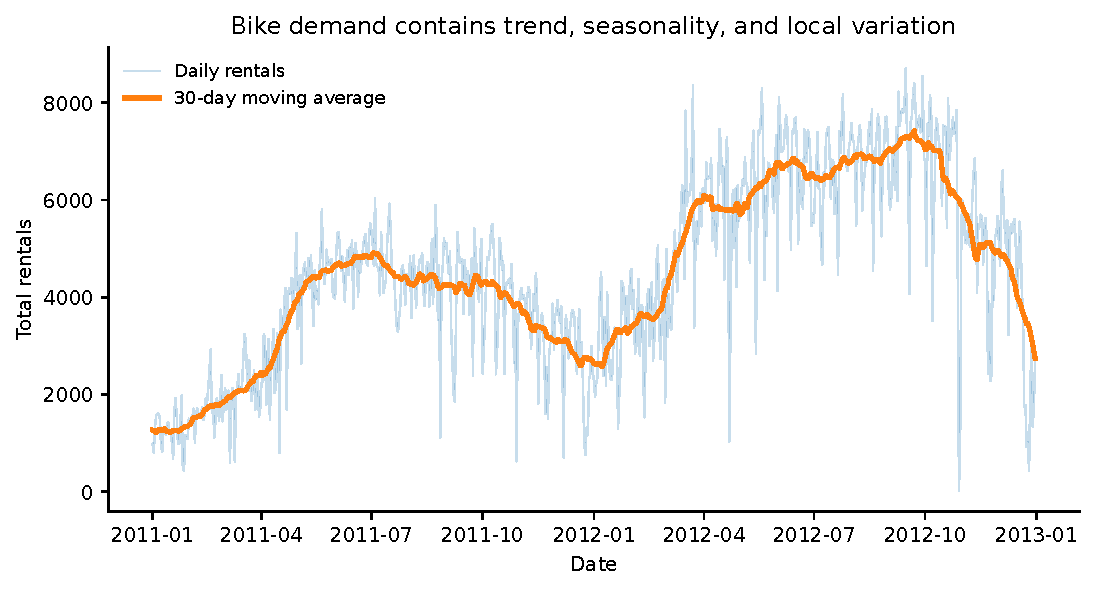
\includegraphics[width=0.88\linewidth]{figures_generated/workflow_bike_daily_pattern.pdf}
\end{utpfig}

In this file, mean demand is about 4,504 rentals per day and normalized temperature has a correlation of about 0.63 with total demand. Neither number is a complete answer. Temperature changes with season, demand changes over calendar time, and working-day status changes the mix of casual and registered users. The workflow therefore moves from a first summary to progressively more careful questions rather than treating the first coefficient as the conclusion.

\begin{keyidea}
The first professional judgment is often not which model to fit, but which comparisons are legitimate given the unit of observation, time ordering, sampling process, and intended claim.
\end{keyidea}

\begin{chapterrecap}
\begin{itemize}
  \item Data science connects questions, data, evidence, and decisions.
  \item Rows are observations; columns are variables with analytical roles.
  \item Inspection comes before transformation or modelling.
  \item Reproducible projects separate raw data, executable code, and outputs.
\end{itemize}
\end{chapterrecap}
